Sketch the root locus showing how the closed loop poles vary with $K$
\begin{center}
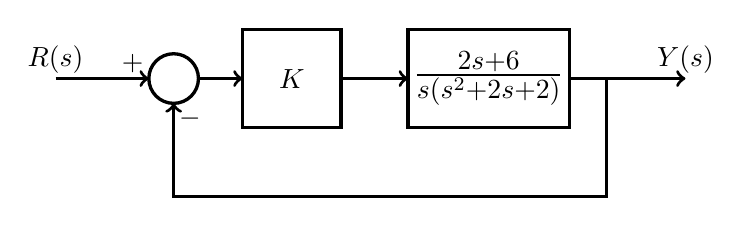
\begin{tikzpicture}[scale=1,inner sep=0pt,outer sep=0pt,very thick,
sysblock/.style={draw,rectangle,inner sep=2pt,minimum width=1.25cm,minimum height=1.25cm,very thick}]
\draw (2,0) node[draw,circle] (sum1) {$\rule{0pt}{18pt}$};
\draw (3.5,0) node[sysblock] (Kp) {$K$};
\draw (6,0) node[sysblock] (G) {\Large $\frac{2s+6}{s(s^{2}+2s+2)}$};
\draw[->] (.5,0) node[above=2pt] {$R(s)$} -- (sum1.180) node[above left=2pt] {$+$};
\draw[->] (sum1.0) --  (Kp);
\draw[->] (Kp) -- (G);
\draw[->] (G) -- ++(2.5,0) node[above=2pt] {$Y(s)$};
\draw[->] (G) ++(1.5,0) -- ++(0,-1.5) -| (sum1.-90) node[below right=2pt] {$-$};
\end{tikzpicture}\end{center}